\subsection{$\PH\to\V\V\to4\ell$ final states}
\label{sec:exotic_h4l}

With the $\chanHZZ$ and $\chanHWW$ decay channels the exotic-spin
$J^P$ hypotheses for the 125 $\GeV$ resonance are tested again the SM
one. In addition, mixed spin-one state hypotheses, as well as the
comprehensive set of spin-two models listed in
Sec.~\ref{sec:phenomenology} are tested. Finally, the fractional
presence of $J^P$ models of a state nearly degenerate in mass with the
SM state are tested.

For these studies, template maximum likelihood fits to the kinematic
discriminants defined in Sec.~\ref{sec:hzzkinematics} are used.  In
the case of $\chanHZZ$ and spin-one, they are
$(\superKD,\psvectorKD,\vectorKD)$. These hypotheses are tested for a
discrete set of values for parameter $f_{b2}$ both for $\qqbar$
production and for generic production, using production-independent
discriminants. All spin-one tests are consistent with the expectation
for the SM Higgs boson.  While the decay-only analysis uses less
information and is expected to provide weaker constraints, the
fluctuations in the observed data lead to stronger constraints for
spin-one models.  The least restrictive result corresponds to the
$1^+$ model in the $\qqbar$ production test with a CL$_s$ value of
$0.031\%$. Any arbitrary spin-one model for the resonance observed in
the $\X\to \PZ\PZ\to 4\ell$ decay mode with any mixture of parity-even
and parity-odd interactions and any production mechanism is excluded
at a CL of 99.97\% or higher. A summary is shown in
Fig.~\ref{fig:jp_summary_1} (left).

In the case of $\chanHWW$ The average separation between the SM Higgs
boson and each alternative spin-1 hypothesis is larger than one
standard deviation. The alternative spin-1 hypotheses are disfavored
with CLs values of 3.9\% for $1^-$, 14.0\% for $1^{+}$, and 8.7\% for
$1_{mix}$. The distribution of the test statistic and the observed
value for the case of $1^-$ against SM is shown in
Fig.~\ref{fig:jp_summary_1} (right).



%%%%%%%%%%%%%%%%%%%%%%%
\begin{figure}[!htbp]
  \begin{center}
\centerline{
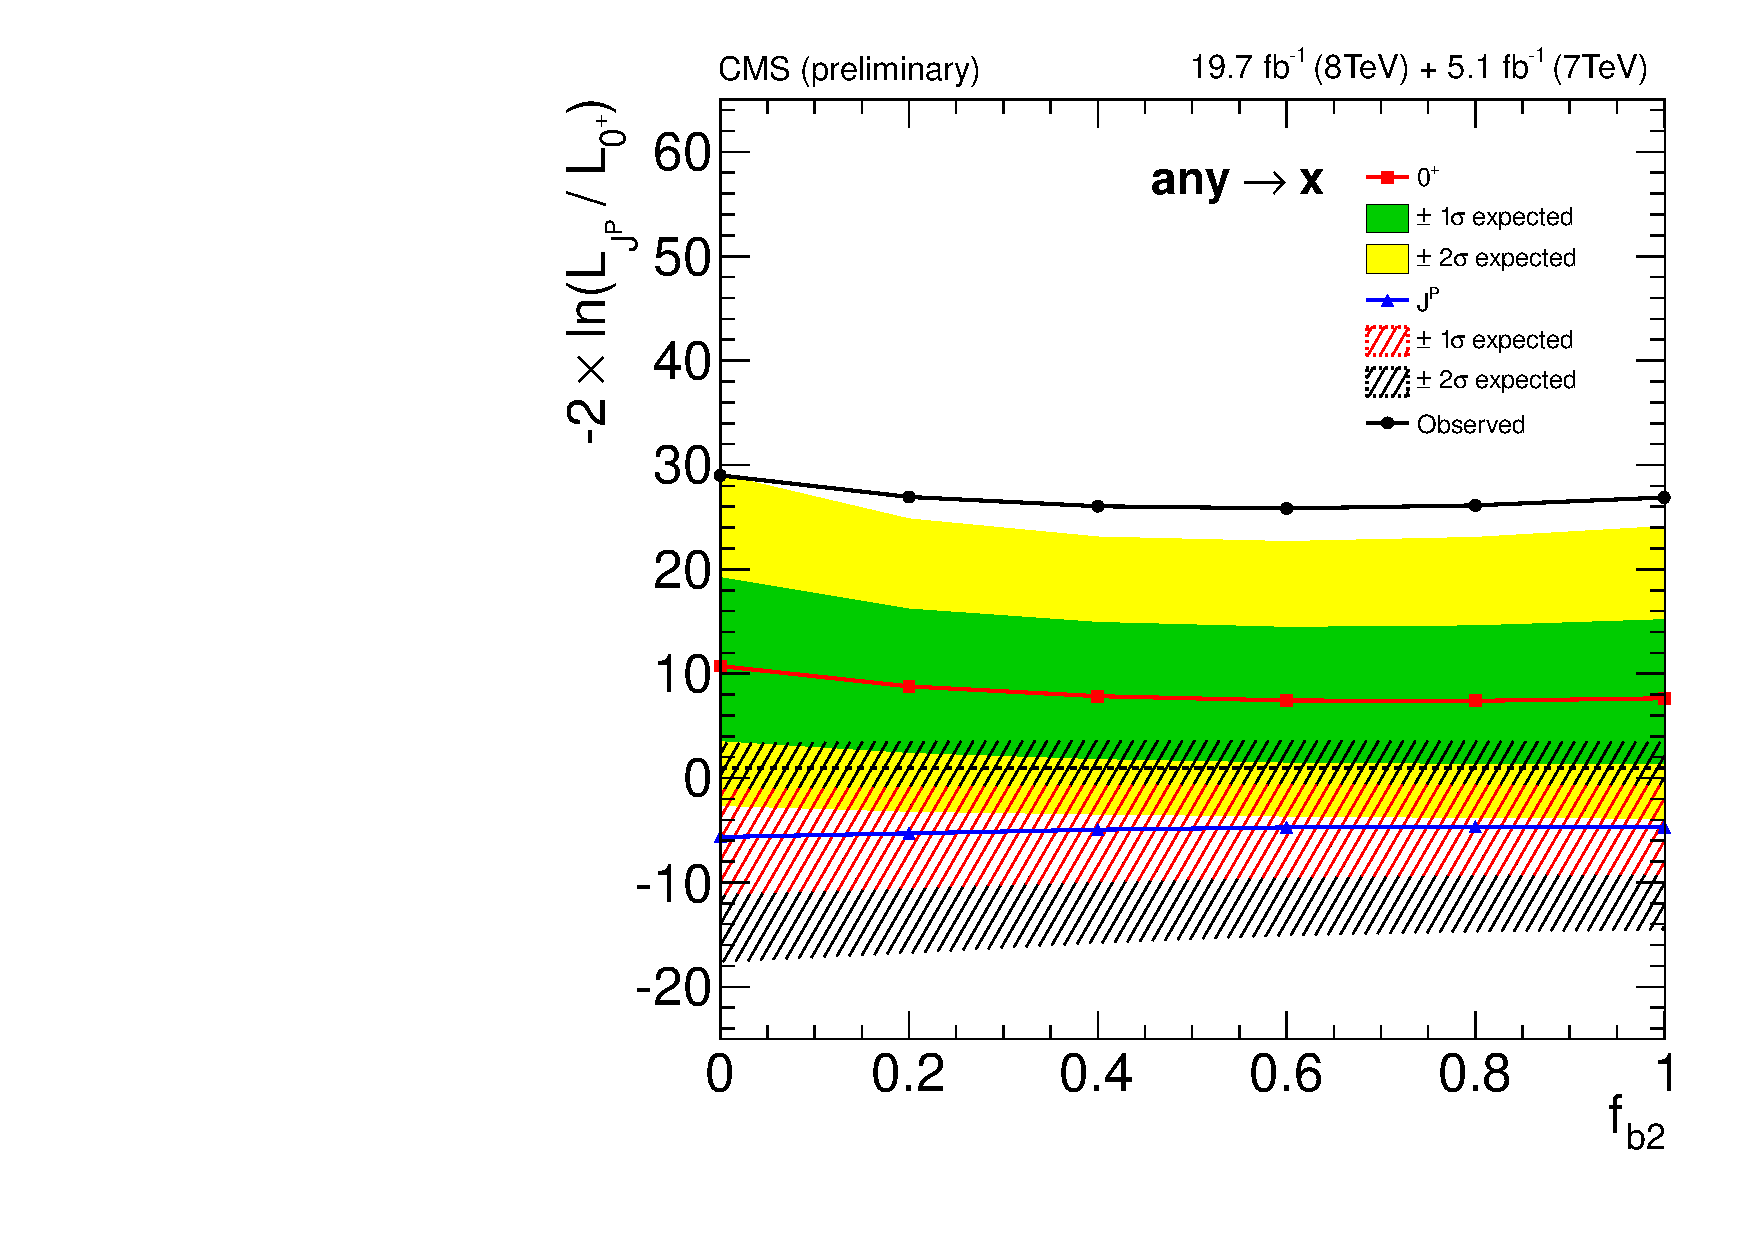
\includegraphics[width=0.49\linewidth]{figures/hzz_spin1_summary_PI.pdf}
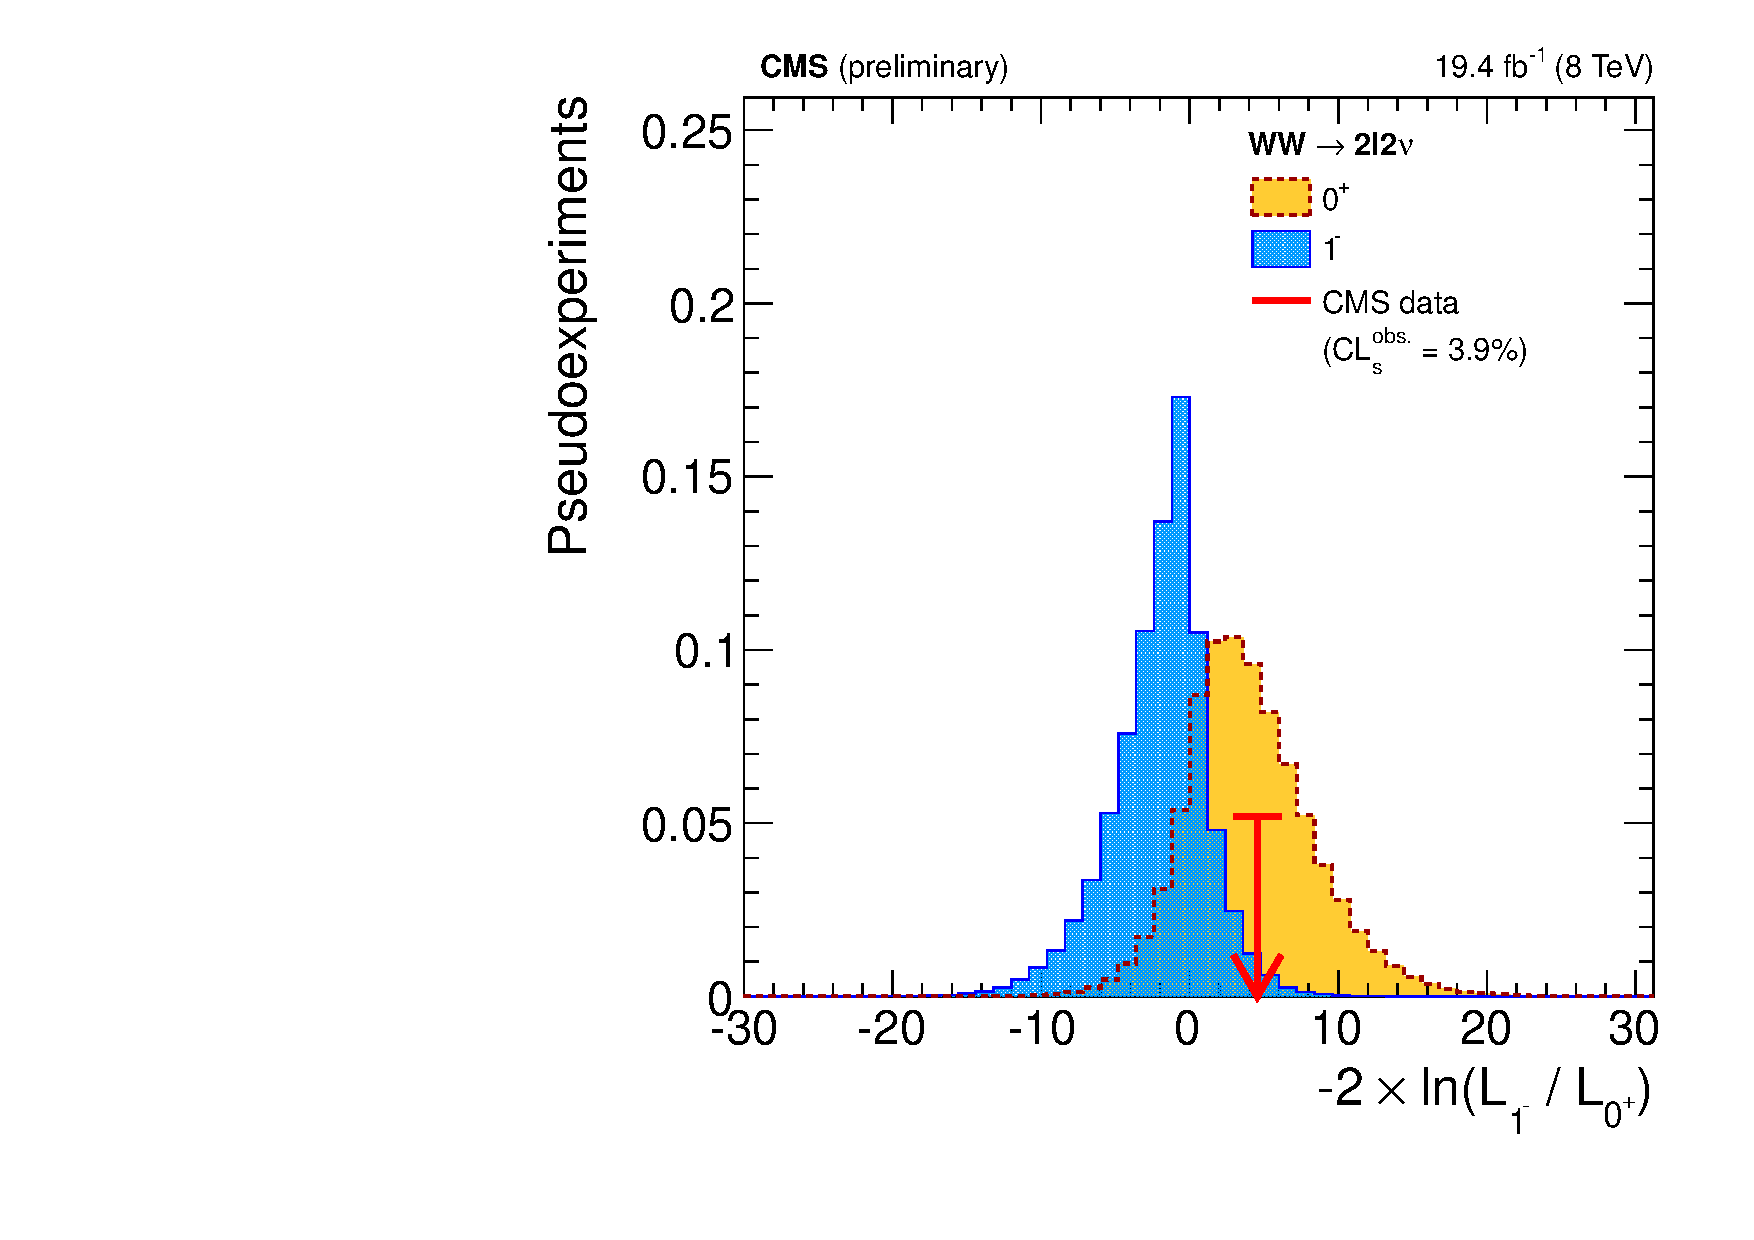
\includegraphics[width=0.52\linewidth]{figures/hzww_spin1_q1minus.pdf}
}
\caption{Left: the expected and observed distributions of median
  test-statistic $q$ for alternative mixed spin-one hypotheses, as
  a function of $f_{b2}$, for $\chanHZZ$, production-independent
  test.  The green and yellow filled bands represent the 1$\sigma$
  and 2$\sigma$ around the median expected value for the SM Higgs
  boson hypothesis. The red and black dashed bands represent the
  1$\sigma$ and 2$\sigma$ around the median expected value for the
  mixed spin-one hypotheses.  Right: Distributions of $-2
  ln(L_{1^-} /L_{0^{+}_{m}})$, combining the 0-jet and 1-jet
  categories, for the $\chanHWW$, channel with $\qqbar$
  production, pure $1^-$ state. The observed value is indicated by
  the red arrow.
  \label{fig:jp_summary_1}} 
  \end{center}
\end{figure}
%%%%%%%%%%%%%%%%%%%%%%%

The hypothesis test of SM Higgs boson against the spin-two resonance
is performed for ten models and three scenarios: $\Pg\Pg$, $\qqbar$
production, and using only decay information in the $\chanHZZ$ decay
channel. Interference between the different amplitude components is
not considered in this case The data disfavor all tested spin-two
hypotheses in favor of the SM hypothesis $0^+$ with $1-$CL$_s$ values
larger than 99\% CL in the case of analysis of decay-only observables.
There are non-zero correlations between the best-fit values obtained
for the various alternate hypotheses.  Measurements are also performed
for two non-interfering states, indicating no evidence for the
presence of a BSM fraction. Fig.~\ref{fig:jp_summary_2} (left) shows the
distribution of the test statistic $q$ for one of these tests
($2_{h2}^+$).

%%%%%%%%%%%%%%%%%%%%%%%
\begin{figure}[!htbp]
\begin{center}
\centerline{
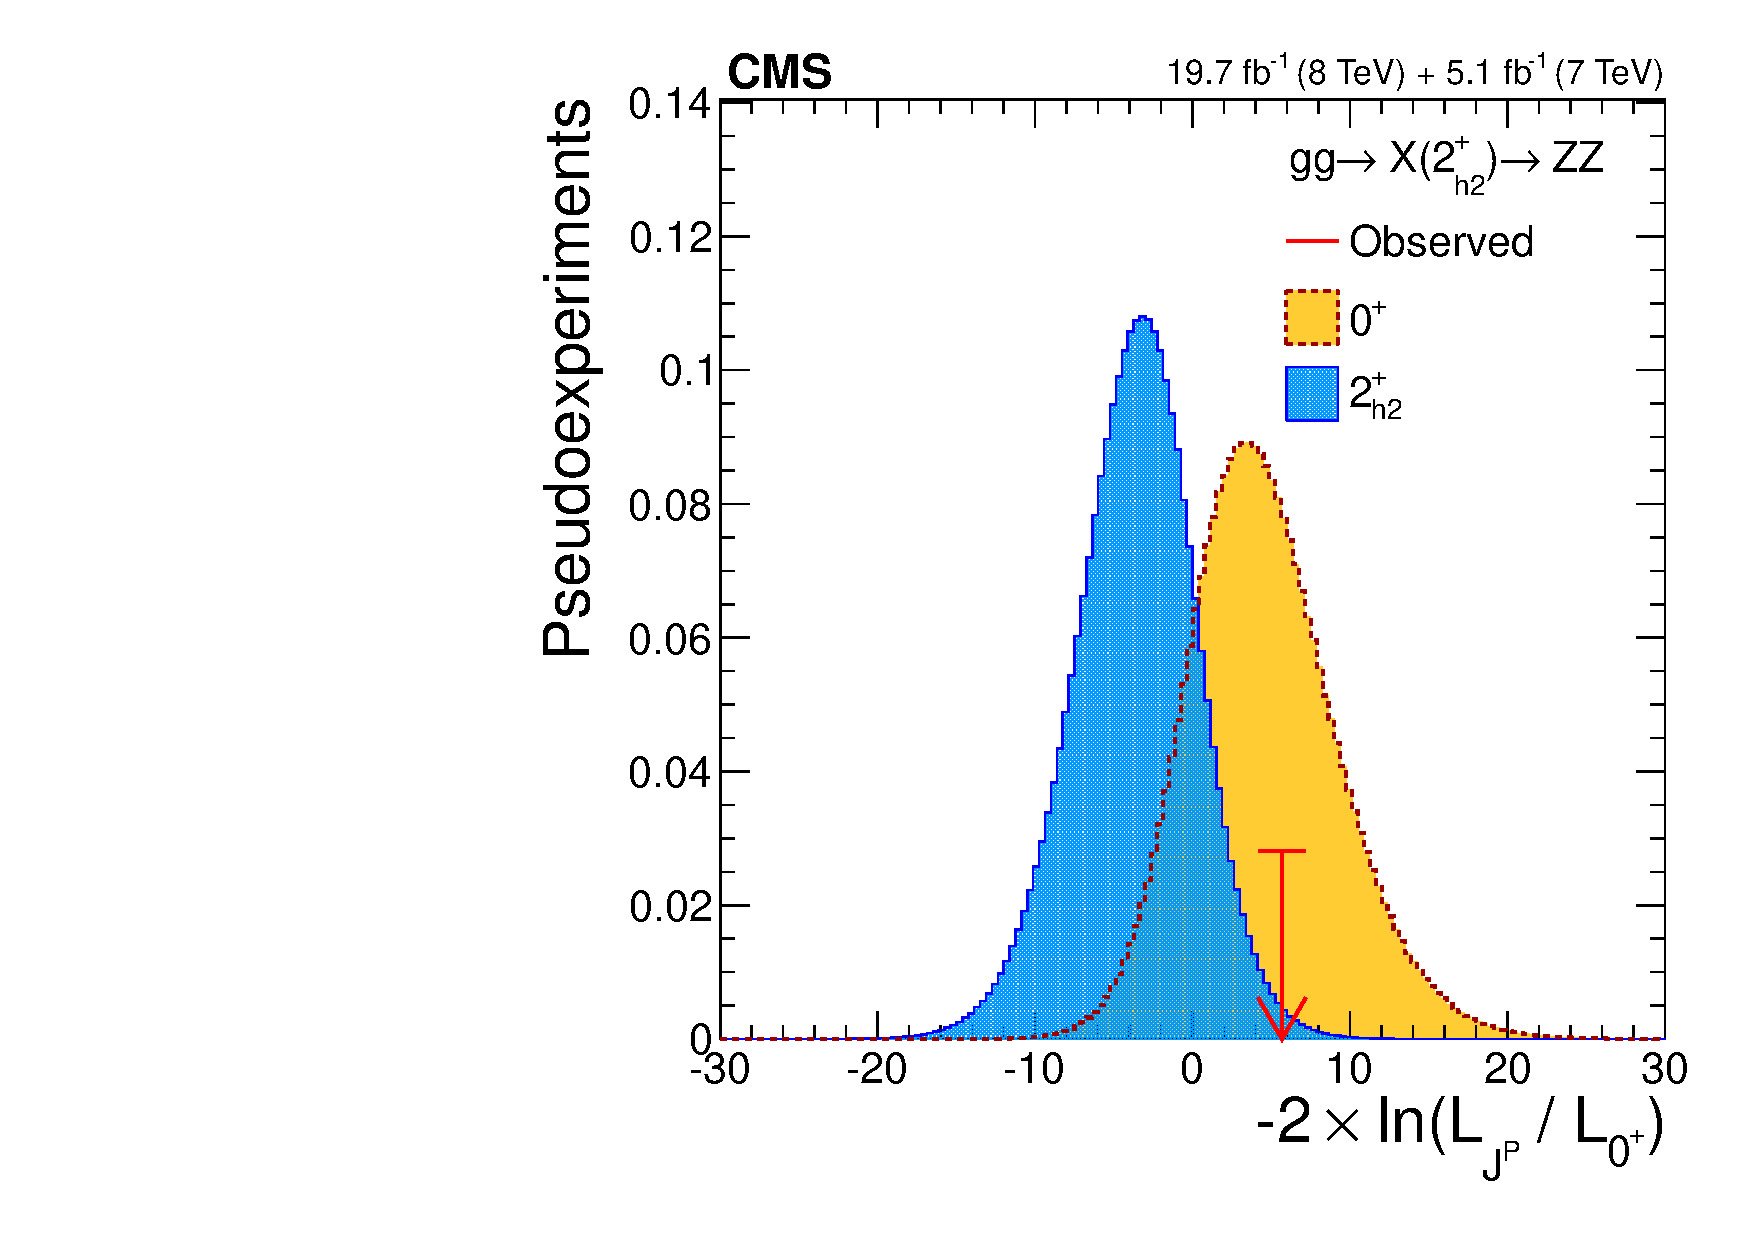
\includegraphics[width=0.45\linewidth]{figures/hzz_sigsep_combine_gg_2h2+.pdf}
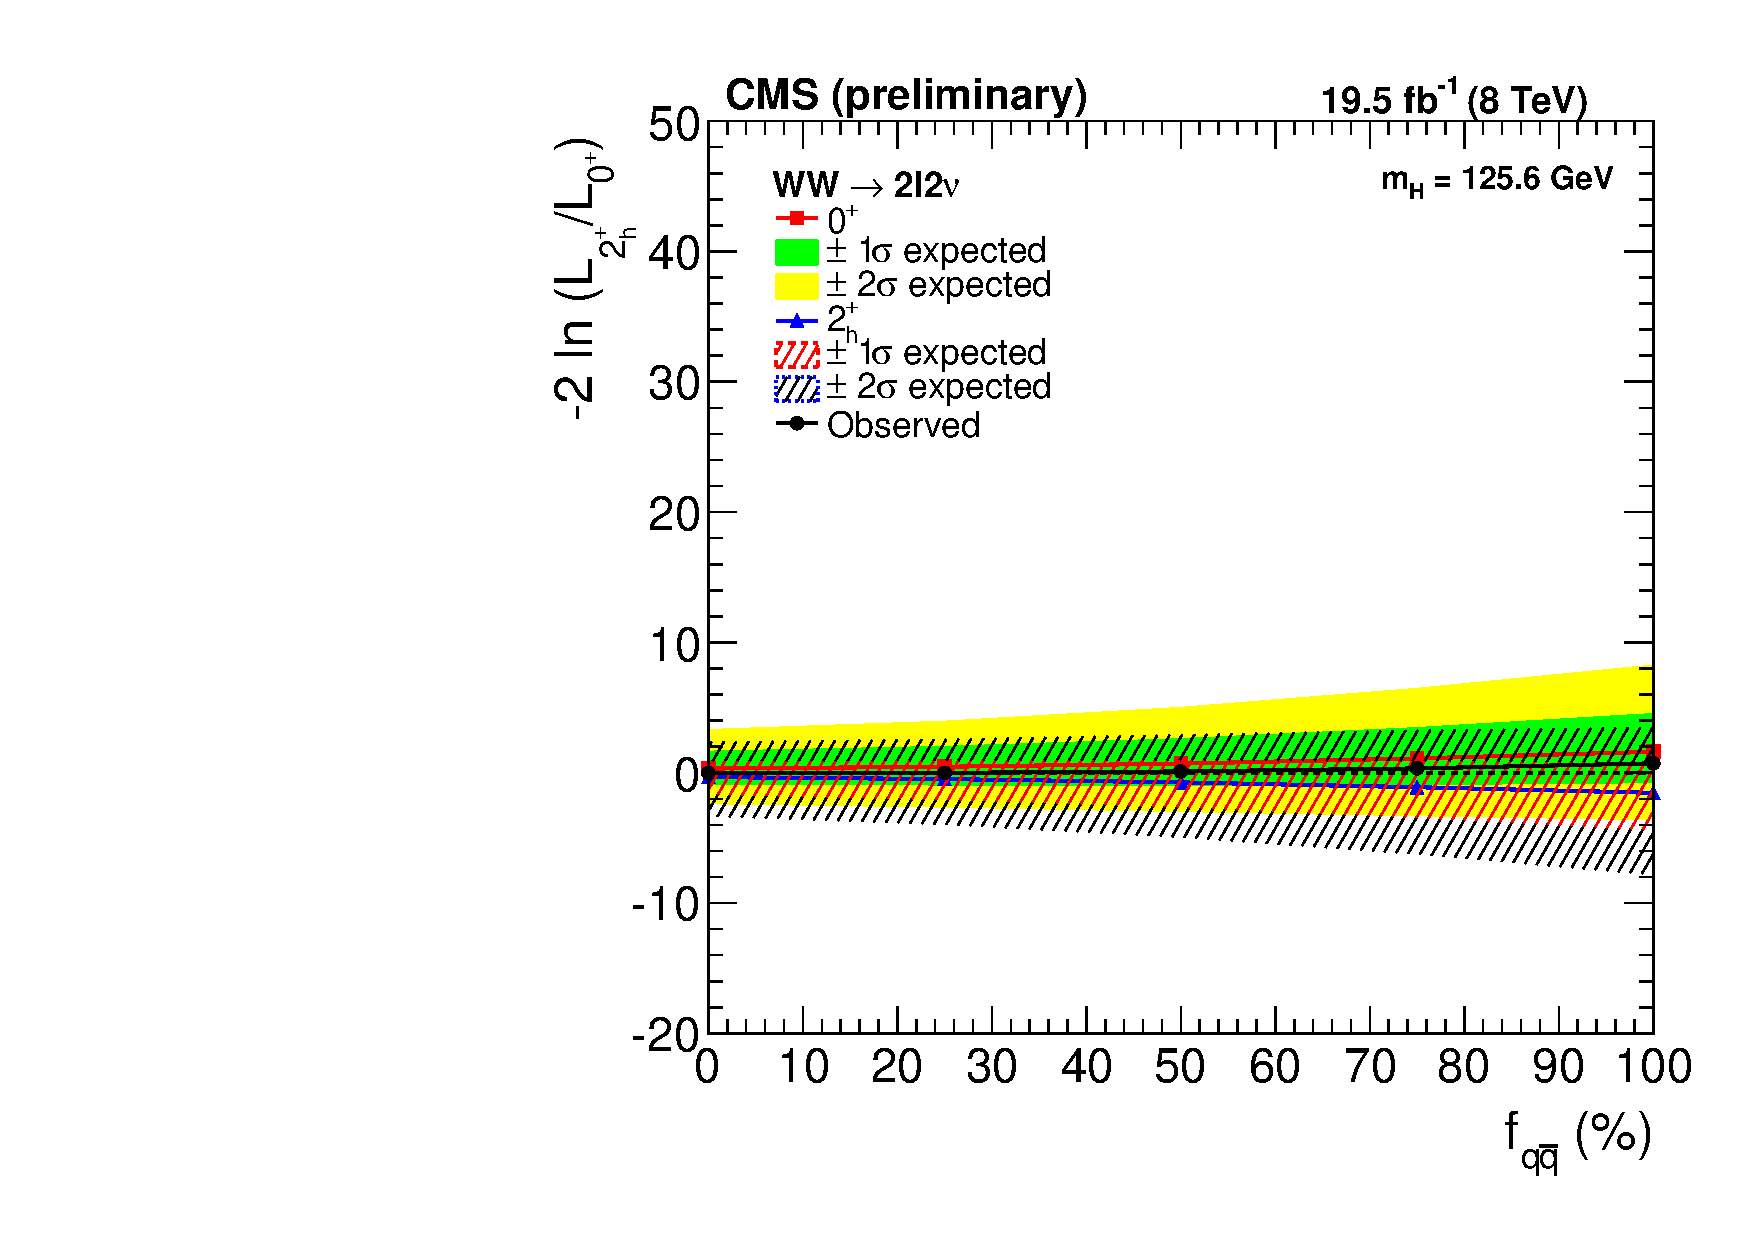
\includegraphics[width=0.45\linewidth]{figures/hww_sigsep_combine_2h2+.pdf}
}
\caption{ Left: Distributions of the test statistic $q=-2\ln({\cal L}_{J^P}/{\cal L}_{0^+})$ 
       for the $J^P=2^+_{h2}$ hypothesis of $\Pg\Pg\to\X(2^+_{h2})\to \PZ\PZ$
      tested against the SM Higgs boson hypothesis ($0^+$). 
            The expectation for the SM Higgs boson is represented by the yellow histogram on the right and the alternative $J^P$ hypothesis by the
      blue histogram on the left. The red arrow indicates the observed $q$ value.  
      Right: Observed and expected median test statistic for the $0^+$ and $\mathrm{J}=2$ hypotheses, as a function of the $f_{q\bar{q}}$ fraction for
      the $J^P=2^+_{h2}$ in the $\chanHWW$ decay mode.
\label{fig:jp_summary_2}}
\end{center}
\end{figure}
%%%%%%%%%%%%%%%%%%%%%%%


The results of the hypothesis testing for the spin-one and spin-two
hypotheses obtained by considering the $\X\to\PZ\PZ\to4\ell$ and
$\X\to\PW\PW\to\ell\nu\ell\nu$ decay channels can be combined, with the
assumption that the same tensor structure for the interactions appears
in both $\X\PZ\PZ$ and $\X\PW\PW$ couplings.  In case of the spin-one
studies, we have tested the models in which the new boson is produced
in the $\qqbar$ process. In case of the spin-two studies, we have
tested the models in which the new boson is allowed to be produced in
both the $\Pg\Pg$ and $\qqbar$ processes.  We have performed these
tests for several choices of the ratio of the two production rates
$f_{\qqbar}$.  The analysis which uses information from the $\chanHZZ$
decay channel is performed in an production-independent way.  Part of
the analysis which is based on the $\chanHWW$ decay channel tests for
several choices of the ratio of the $f_{\qqbar}$ ratio explicitly.
The expected separations from the test statistic distributions for all
the considered models are summarized in 
Figure~\ref{fig:jp_summary_comb}. The data disfavor all tested
spin-one and spin-two hypotheses in favor of SM hypothesis $0^+$ with
CL$_s$ value larger then 99.9\% CL. Each of these exclusions is tested
and reported independently of the other hypotheses, but one should
note that there are correlations between the various alternate
hypotheses.

%%%%%%%%%%%%%%%%%%%%%%%
\begin{figure}[!htbp]
  \begin{center}
    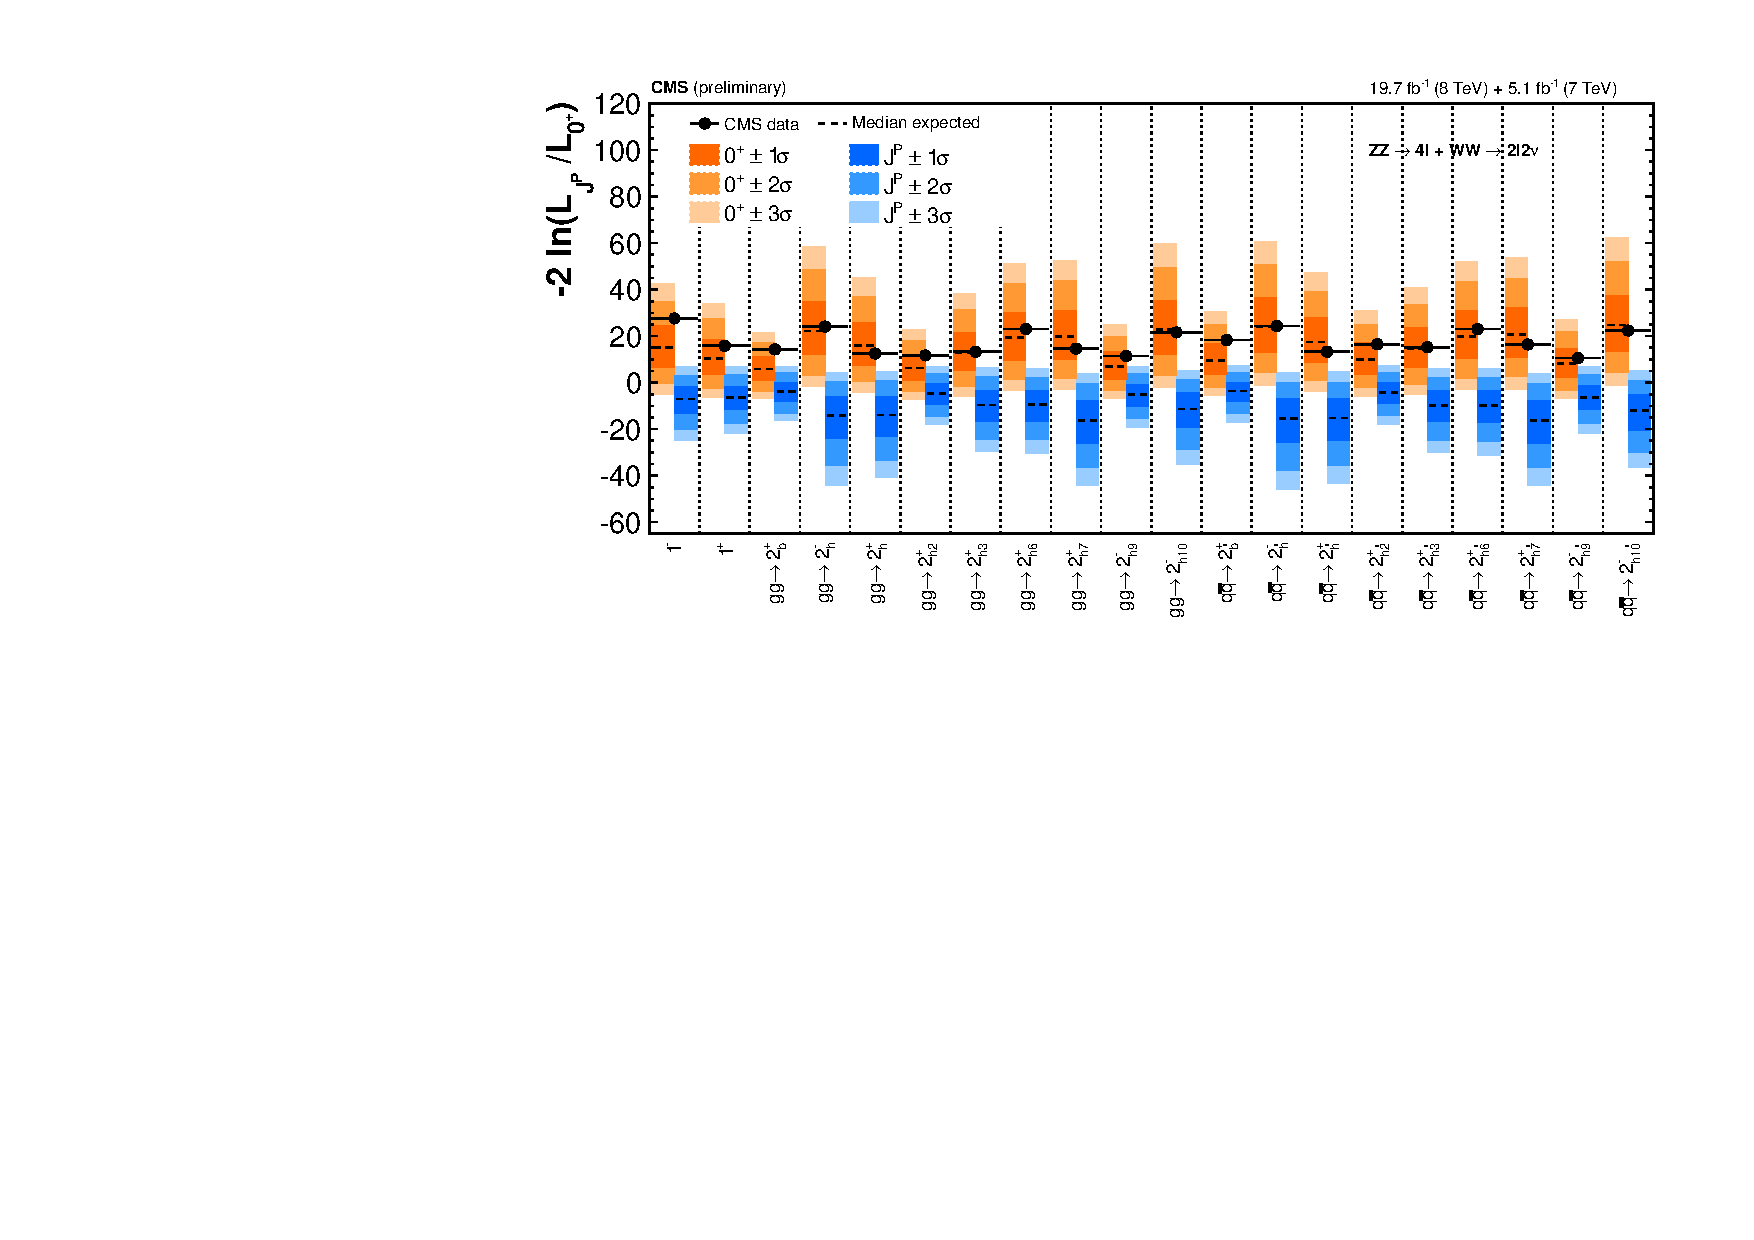
\includegraphics[width=0.95\linewidth]{figures/JP_SummaryPlot.pdf}
    \caption{
     Summary of the expected and observed values for the
      test-statistic $q$ distributions for the alternative spin-one and spin-two
      hypotheses tested with respect to the SM Higgs boson, based on the 
     combined analysis in $\chanHZZ$ and 
     $\chanHZZ$ decay channels.  The
      orange (blue) bands represent the 1$\sigma$, 2$\sigma$, and
      3$\sigma$ around the median expected value for the SM Higgs
      boson hypothesis (alternative hypothesis). The black point
      represents the observed value.
      \label{fig:jp_summary_comb}} 
  \end{center}
\end{figure}
%%%%%%%%%%%%%%%%%%%%%%%


\subsection{$\PH\to\Pgg\Pgg$ final state}
\label{sec:exotic_hgg}

Figure~\ref{fig:hgg_spin2} (left) shows the distribution of the
expected signal strength, $\mu$, relative to the SM expectation in the
five bins of $\abscostheta$ for the SM, and for two $2_m^+$ models:
where the $2_m^+$ resonance is produced entirely by gluon-fusion
($\Pg\Pg$), and where it is produced entirely by quark-antiquark
annihilation ($\Pq\Paq$).  The hypothesis of SM Higgs boson is
tested against two alternative models of a $2_m^+$ resonance produced
entirely by either gluon-fusion, or entirely by quark-antiquark
annihilation, or by three intermediate mixtures of $\Pg\Pg$ and
$\Pq\Paq$ spin-2 production, with a fraction of cross section
$f_{\qqbar}$. Figure~\ref{fig:hgg_spin2} (right) shows the values of
the test statistic as a function of $f_{\qqbar}$.  The hypothesis of the
signal being $2_m^+$ is disfavored for all values of $f_{\qqbar}$
tested.


\begin{figure}[!hbtp]
  \begin{center}
    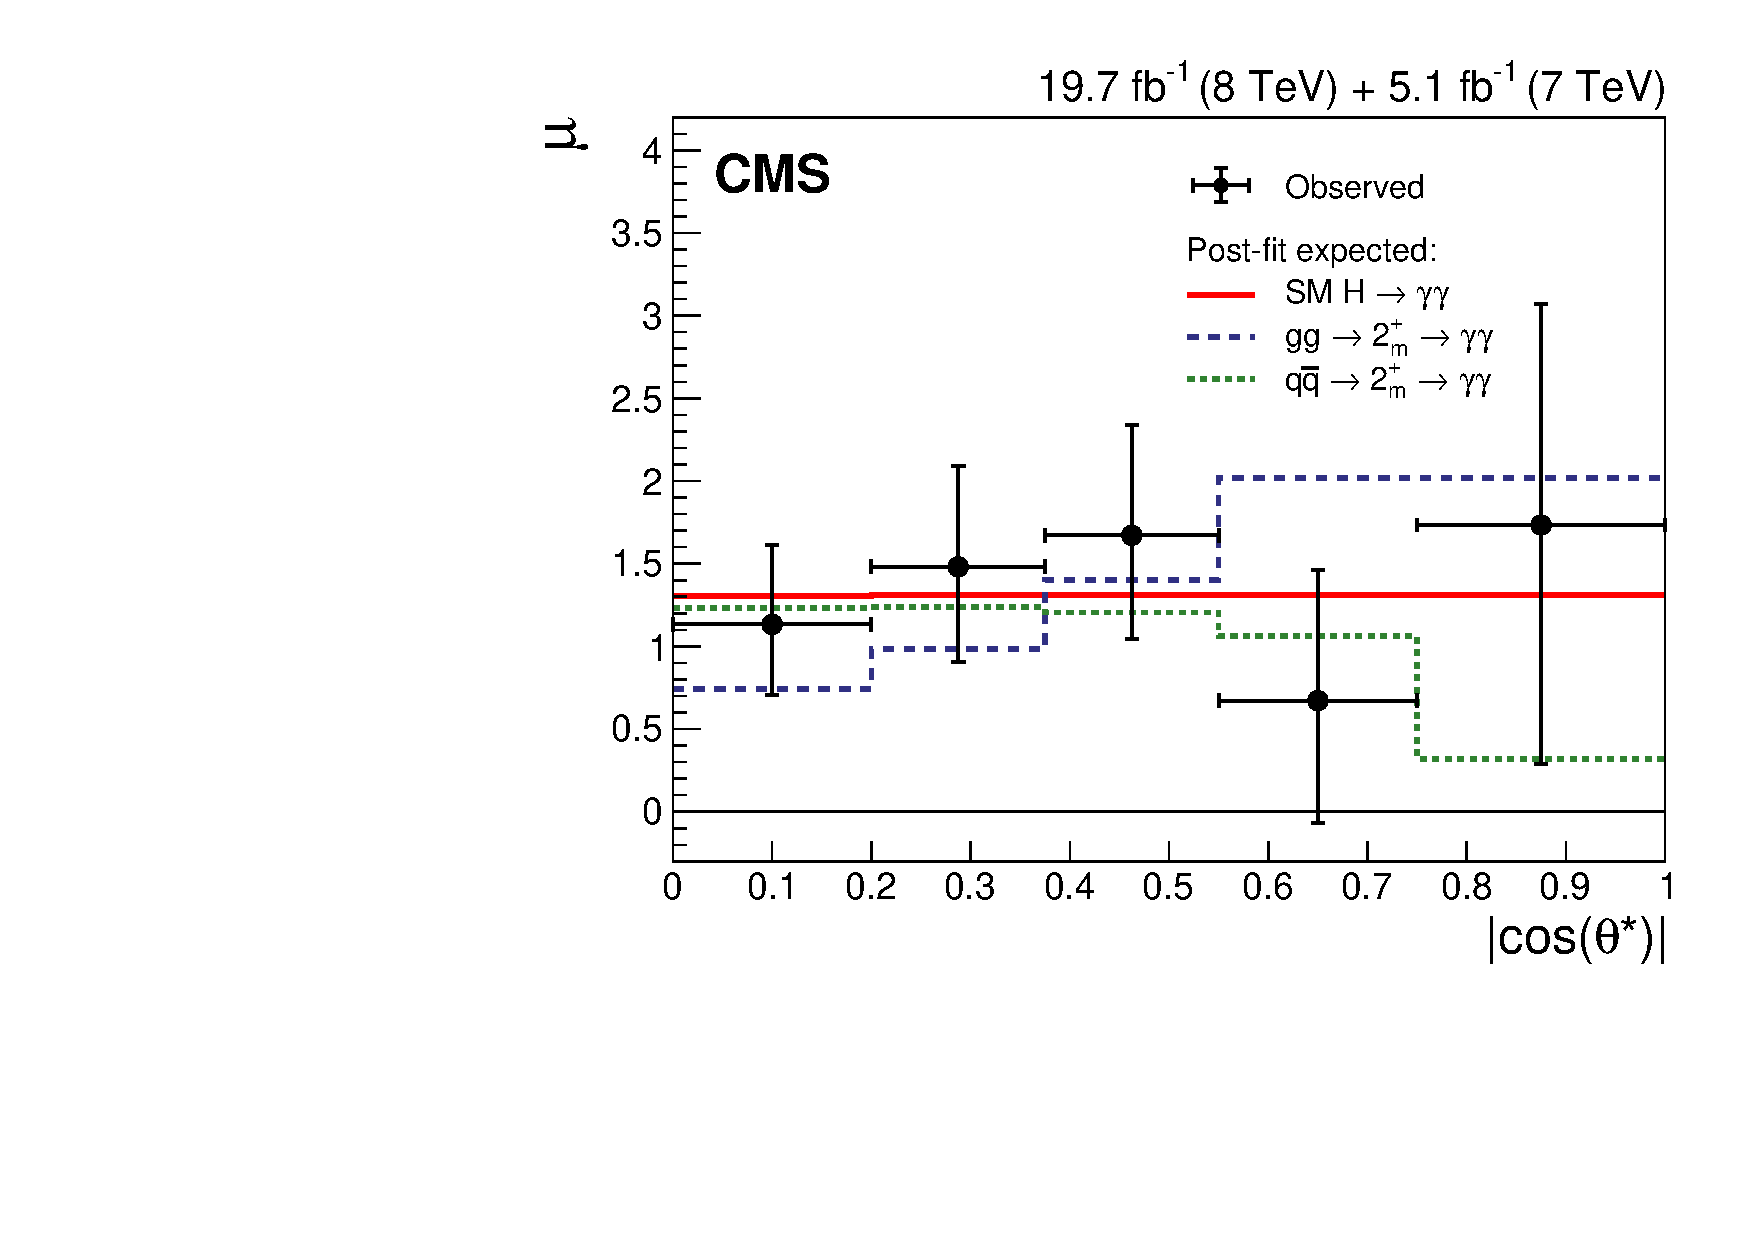
\includegraphics[width=0.49\linewidth]{figures/hgg_mucosth.pdf}
    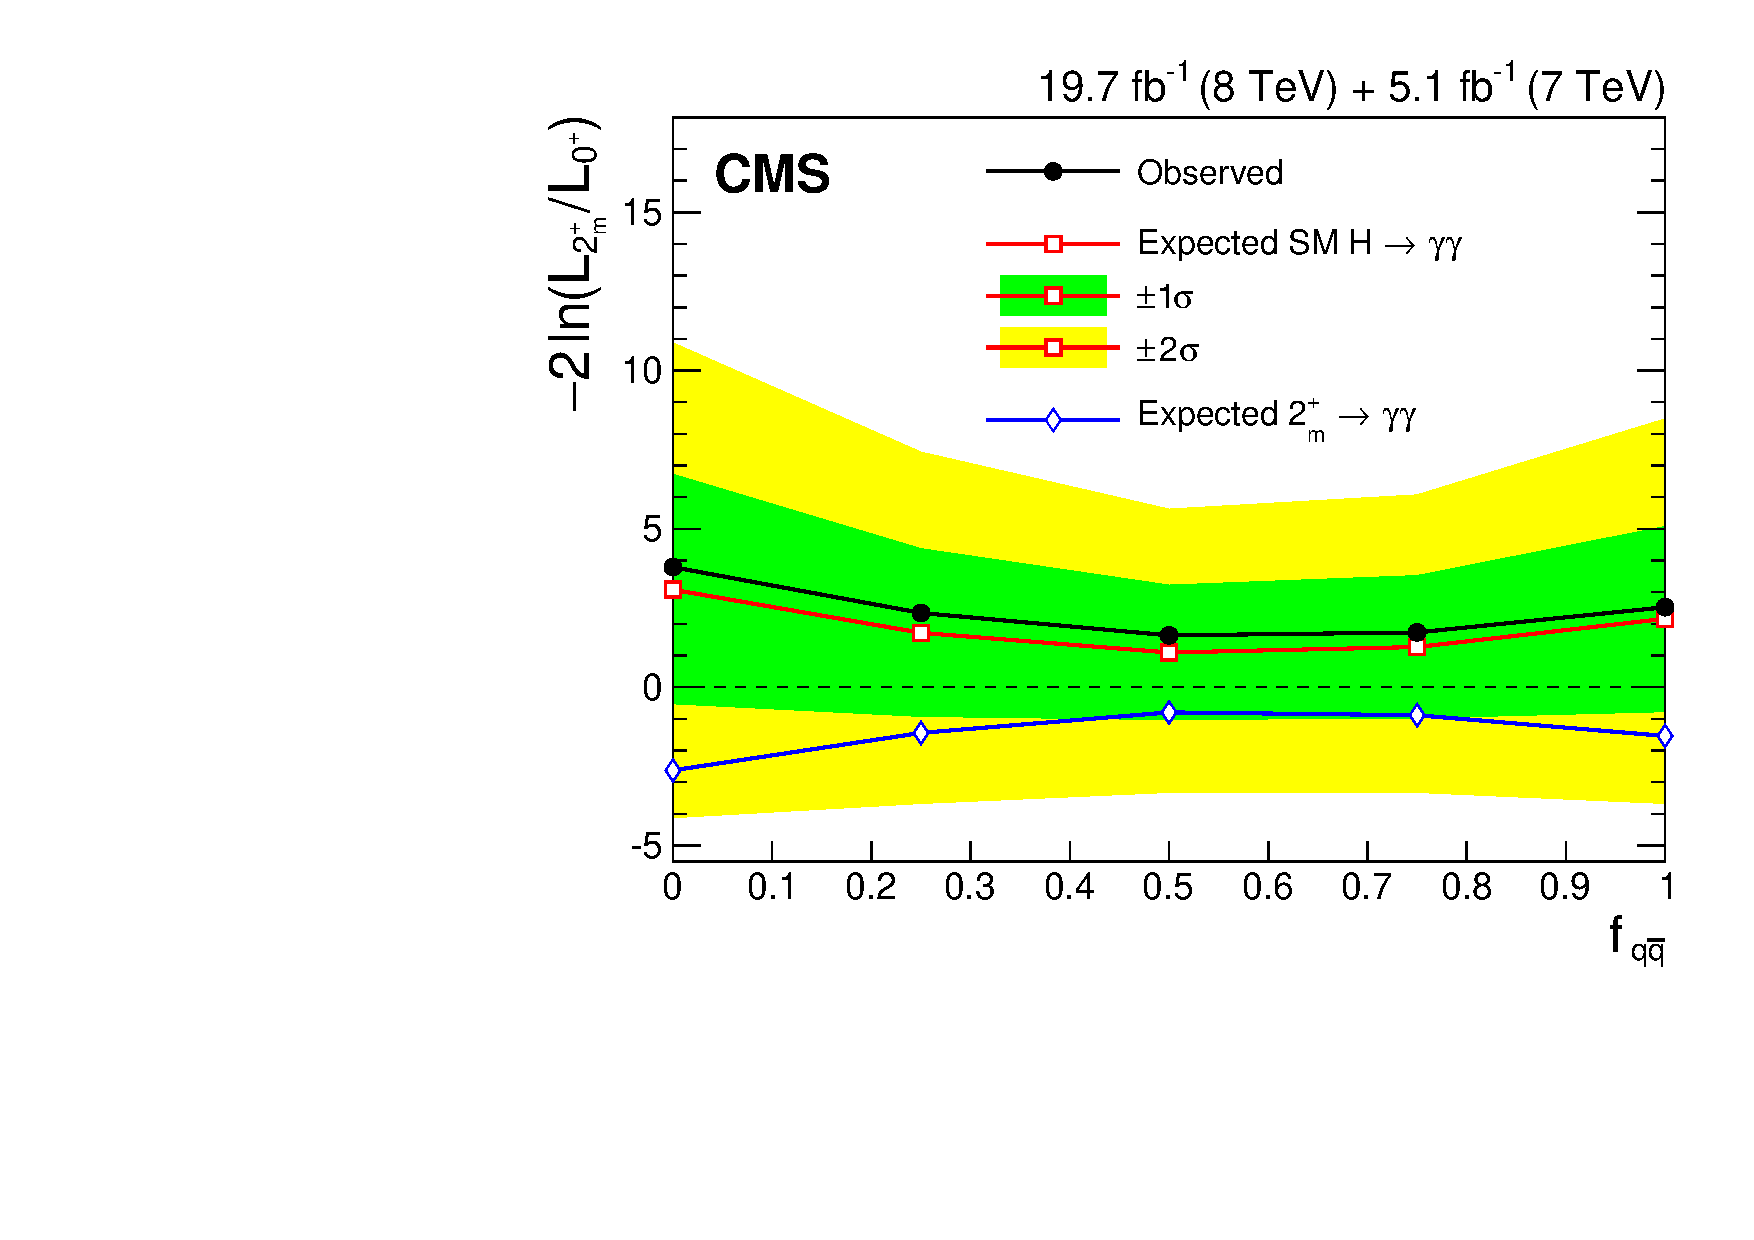
\includegraphics[width=0.49\linewidth]{figures/hgg_spin2_excl.pdf}
    \caption{Top: Signal strength in five bins of $\abscostheta$ expected for SM, for $2^+_m$ produced
      by $\Pg\Pg$, and for $2^+_m$ produced by $\qqbar$.
      The signal strength observed in the data is shown by the black points.
      Right: Test statistic for pseudo-experiments generated under the SM hypothesis (open squares) and the
$2^+_m$, hypothesis (open diamonds), as a function of the $f_{\qqbar}$ fraction.
      The observed distribution in the data is shown by the black points.
      \label{fig:hgg_spin2}
    }
  \end{center}
\end{figure}



